\subsection{Ventilations}
%\label{sec:ventilationsberegninger}

%\subsection{Beregning af indblæsning}
%\label{sub:indblaesning_beregning}
\subsubsection{Tryktab i indblæsning} \label{sub:tryktab_indblaesning}
I tabel \ref{table:oversigt_l_indblaesning}, beskriver længderne brugt til indblæsningen. 
Lufthastighed, Tryktab per meter beskrevet i tabellen er fundet ved hjælp af lindab's App `Vent Tools',
og tryktabet er herefter udregnet fra de tal.
\begin{table}[h!]
    \begin{center}
       \begin{tabular}{|l|r|r|r|r|r|}
           \hline
           Længde & meter & q$_{v}$ & V & P$_{a}$ / m & Tryktab\\
           \hline
            P & 3,94 m & 13,61 m$^3$/t & 0,19 m/s & 0,0 P$_{a}$/m & 0 Pa\\
            O & 0,74 m & 13,61 m$^3$/t & 0,19 m/s & 0,0 P$_{a}$/m & 0 Pa\\
            N & 4,71 m & 56,49 m$^3$/t & 0,78 m/s & 0,1 P$_{a}$/m & 0,471 Pa\\
            M & 4,24 m & 12,96 m$^3$/t & 0,18 m/s & 0,0 P$_{a}$/m & 0 Pa\\
            K & 3,50 m & 25,81 m$^3$/t & 0,36 m/s & 0,0 P$_{a}$/m & 0 Pa\\
            J & 1,78 m & 82,30 m$^3$/t & 1,14 m/s & 0,1 P$_{a}$/m & 0,178 Pa\\
            I & 0,74 m & 82,30 m$^3$/t & 1,14 m/s & 0,1 P$_{a}$/m & 0,074 Pa\\
           \hline
       \end{tabular}
   \end{center}
   \caption{Oversigt over længderne brugt i indblæsning}
   \label{table:oversigt_l_indblaesning}
\end{table}

Tryktabet i T-stykkerne er beskrevet i tabel \ref{table:oversigt_tryktab_t-roer_ind}. 
Lufthastighed for Stue/Alrum/Køkken og Værelse 1 er beregnet ud fra ligning \ref{eqn:omregning_vs_til_lh} på side \pageref{eqn:omregning_vs_til_lh}.
Stue's udregning kan se i udregning \ref{eqn:udregning_af_vs_stue}.
\begin{align} \label{eqn:udregning_af_vs_stue}
    V     &= \frac{ q_v \cdot 4 }{ d_{n}^{2} \cdot \pi \cdot 3600 } \nonumber \\
    V     &= \frac{ 42,88 \cdot 4 }{ (160/1000)^{2} \cdot \pi \cdot 3600 } \nonumber \\
    V     &= \frac{ 171,53 }{ 92,16 \cdot \pi } \nonumber \\
    V     &= 0,592 \text{ m/s}
\end{align}
Når der aflæses i databladet for T-stykkerne, så er det udenfor skalaen.
Det kommer af, at rørdiameteren er sat efter udsugning det sætter lufthastigheden ned og derfor kan tabet sættes til 0 Pa.
Det betyder, at indblæsningen ikke ville have noget tab af betydning i T-stykkerne.
\begin{table}[h!]
    \begin{center}
       \begin{tabular}{|l|r|r|r|}
           \hline
           T-rør & V$_{1}$ & V$_{2}$ & Tryktab \\
           \hline
           T$_{\text{J->N}}$ & 1,14 m/s & 0,78 m/s & 0 Pa \\ 
           T$_{\text{J->K}}$ & 1,14 m/s & 0,36 m/s & 0 Pa \\ 
           T$_{\text{N->O}}$ & 0,78 m/s & 0,19 m/s & 0 Pa \\ 
           T$_{\text{N->Stue}}$ & 0,78 m/s & 0,59 m/s & 0 Pa \\ 
           T$_{\text{K->M}}$ & 0,36 m/s & 0,18 m/s & 0 Pa \\ 
           T$_{\text{K->Værelse 1}}$ & 0,36 m/s & 0,71 m/s & 0 Pa \\ 
           \hline
       \end{tabular}
   \end{center}
   \caption{Oversigt tryktabet i T-rør for indblæsning}
   \label{table:oversigt_tryktab_t-roer_ind}
\end{table}
Nu kan tabet findes på den længeste strækning. Som er på indblæsning er soveværelset.
\begin{table}[h!]
    \begin{center}
       \begin{tabular}{lcr}
           \hline
           \hline
           \textbf{Soveværelse} &  & \\
           \hline
           \hline
           Ventil (6mm åbning) & : & 15,000 Pa \\
           90$^\circ$ BU    & : & 0 Pa \\
           Rør$_{\text{P}}$ & : & 0 Pa \\
           90$^\circ$ BU    & : & 0 Pa \\
           Rør$_{\text{O}}$ & : & 0 Pa \\
           T-Stykke$_{\text{N->O}}$  & : & 0 Pa\\
           Rør$_{\text{N}}$ & : & 0,471 Pa \\
           T-Stykke$_{\text{J->N}}$  & : & 0 Pa\\
           Rør$_{\text{J}}$ & : & 0,178 Pa \\
           90$^\circ$ BU    & : & 3,800 Pa \\
           Rør$_{\text{I}}$ & : & 0,074 Pa \\
           \hline
           Samlet tryktab & : & \underline{\underline{ 19,523 Pa}} 
       \end{tabular}
   \end{center}
   %\caption{Oversigt tryktabet i T-rør}
   %\label{table:oversigt_tryktab_t-roer}
\end{table}


%\subsection{Beregning af udsugning}
%\label{sub:udsugning_beregning}

\subsubsection{Tegning over ventilationsrør} \label{fig:tegning_ventr}
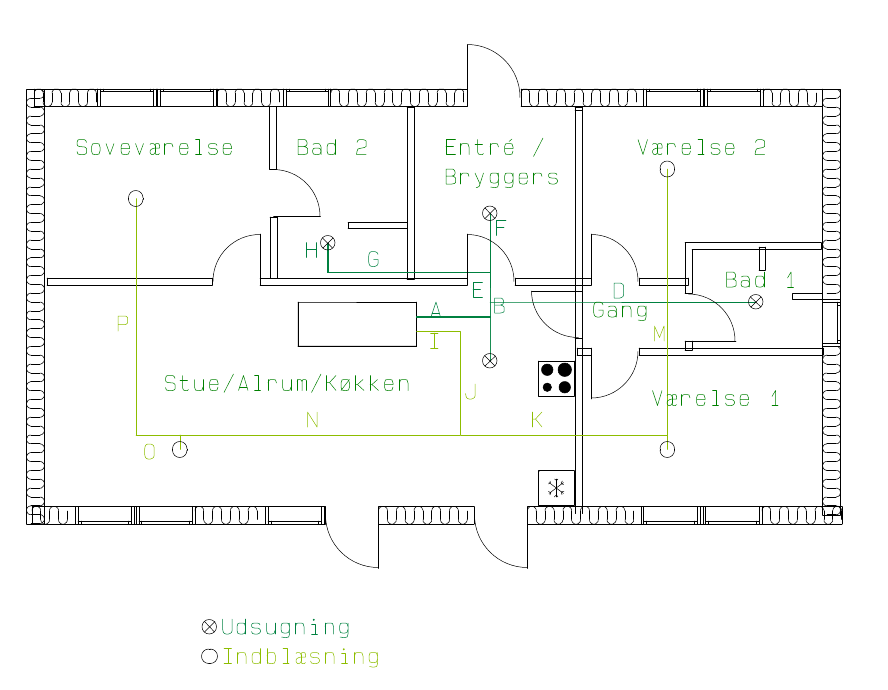
\includegraphics[scale=0.60,angle=90,origin=c]{appendix/ventilation/ventilation_tegning.png}%{appendix/ventilation/plantegning2.pdf}